\documentclass[a4paper,14pt]{extarticle}

\usepackage{geometry}
\geometry{a4paper,tmargin=2cm,bmargin=2cm,lmargin=3cm,rmargin=1cm}
\usepackage[T2A]{fontenc}
\usepackage[utf8]{inputenc}
\usepackage[english,main=russian]{babel}
\usepackage{indentfirst}
\usepackage{graphicx}
\graphicspath{{./images/}}
\usepackage{setspace}
\linespread{1.3}
\usepackage{tempora}
\usepackage{amsmath}
\usepackage{booktabs}
\usepackage{array}
\usepackage{caption}
\usepackage{hyperref}
\hypersetup{unicode=true,hidelinks}
\usepackage{listings}

\sloppy
\clubpenalty=10000
\widowpenalty=10000



\lstset{basicstyle=\ttfamily\small,breaklines=true,
  columns=fullflexible,frame=single,numbers=none,
  showstringspaces=false,tabsize=4,captionpos=t,keepspaces=true}
\renewcommand{\lstlistingname}{Листинг}
\lstdefinelanguage{Go}{
morekeywords={package,import,func,type,struct,return,if,else,for,range,go,defer,
chan,make,map,var,const,select,case,break,continue},
morecomment=[l]{//},morestring=[b]"
}
\begin{document}

\begin{titlepage}
\thispagestyle{empty}

\vspace*{-60pt}

\hspace*{-82pt}
\begin{minipage}{0.3\textwidth}
\centering
\IfFileExists{images/emblem.png}{%
  
\includegraphics[width=0.9\textwidth]{emblem.png}%
}{%
  \IfFileExists{images/emblem.jpg}{%
    \includegraphics[width=0.9\textwidth]{emblem.jpg}%
  }{}%
}
\end{minipage}
\begin{minipage}{0.67\textwidth}
\small
\textbf{
\vspace*{-0.7ex}
\centerline{Министерство науки и высшего образования Российской Федерации}
\vspace*{-0.7ex}
\centerline{Федеральное государственное бюджетное образовательное учреждение}
\vspace*{-0.7ex}
\centerline{высшего образования}
\vspace*{-0.7ex}
\centerline{<<Московский государственный технический университет}
\vspace*{-0.7ex}
\centerline{имени Н. Э. Баумана}
\vspace*{-0.7ex}
\centerline{(национальный исследовательский университет)>>}
\vspace*{-0.7ex}
\centerline{(МГТУ им. Н. Э. Баумана)}
}
\end{minipage}

\vspace{-25pt}
\hspace{-35pt}\rule{\textwidth}{2.3pt}

\vspace*{-20.3pt}
\hspace{-35pt}\rule{\textwidth}{0.4pt}

\vspace{1.5ex}
\hspace{-35pt}\noindent\small
ФАКУЛЬТЕТ\hspace{80pt} <<Информатика и системы управления>>

\vspace*{-16pt}
\hspace{47pt}\rule{0.83\textwidth}{0.4pt}

\vspace{0.5ex}
\hspace{-35pt}\noindent\small
КАФЕДРА\hspace{50pt} <<Теоретическая информатика и компьютерные технологии>>

\vspace*{-16pt}
\hspace{30pt}\rule{0.866\textwidth}{0.4pt}

\vspace{11em}

\begin{center}
\Large \textbf{Лабораторная работа №4} \\
\large \textbf{по курсу <<Параллельные и распределённые системы>>} \\
\large <<Синхронизация и пулы потоков>>
\end{center}

\normalsize

\vspace{8em}

\begin{flushright}
Студент группы ИУ9-51Б \\
Шалимов Д. И. \\
\vspace{2ex}
Преподаватель Царев А.С.
\end{flushright}

\bigskip
\vfill

\begin{center}
\textsl{Москва 2026}
\end{center}
\end{titlepage}

\setcounter{page}{2}
\tableofcontents
\newpage




\section{Постановка задачи}
Я выполнил задачи 1 и 3: эволюцию клеточного поля с барьерной
синхронизацией, решето Эратосфена, факториал и число Фибоначчи с пулом
работников. Решение написано на Go, чтобы вычисления могли исполняться
параллельно без ограничения GIL Python.

В задаче 1 поле делится на полосы строк. Каждый работник читает только
свою полосу, а недостающие строки запрашивает у соседей.
Новое поколение записывается отдельно, затем копируется в исходное.
На каждом шаге работники синхронизируются барьерами.
Поле замкнуто в тор. Требуется сравнить время шага с последовательным.
В задаче 3 требуется сравнить время трёх вычислений без пула и при
разном числе работников. Задача 2 в работу не включена.

\section{Структура программы}
Я разделил работу на две независимые программы:
\texttt{task1/main.go} содержит только задачу эволюции;
\texttt{task3/main.go} --- численные задачи с пулом.
У каждой свой \texttt{main}, флаг проверки и файл измерений.
Они запускаются по отдельности, не импортируют друг друга.
Общий \texttt{plot.py} нужен только для построения рисунков.

\section{Реализация}
\subsection{Эволюция}
Клетка становится живой при трёх живых соседях. При двух соседях
выживает только уже живая клетка; в остальных случаях она пуста.
Учитываются восемь позиций вокруг клетки.
Индекс соседнего столбца берётся по модулю ширины, а соседней полосы ---
по модулю числа работников.

Работнику передаётся копия непрерывного диапазона строк. Размеры полос
отличаются не более чем на одну строку.
На каждом шаге работник отправляет запрос предыдущему на последнюю
строку и следующему --- на первую. Запрос содержит канал ответа.
Затем работник обслуживает два встречных запроса, отправляя копии
своих строк, и получает две границы.
Каналы запросов буферизованы на два сообщения, ответов --- на одно.
Это позволяет сначала отправить запросы, а затем обслужить их.
Прямого чтения чужой матрицы нет.

После вычисления новой полосы первый барьер ждёт всех работников.
Затем новые строки копируются в исходные, второй барьер ждёт завершения
копирования перед следующим шагом.
Повторно используемый барьер реализован через \texttt{sync.Cond},
счётчик пришедших и номер фазы.
Последний участник меняет фазу и вызывает \texttt{Broadcast};
остальные ожидают смены фазы в цикле.
Главный поток ждёт завершения через \texttt{sync.WaitGroup}.

\subsection{Пул}
Функция \texttt{pool} создаёт фиксированное число goroutine.
Они получают функции-задачи из канала, выполняют их и после закрытия
канала завершаются. Ответы записываются в разные элементы массива
и читаются главным потоком только после \texttt{Wait}.
Внутри задач нет ожидания дочерних задач этого же пула.

Goroutine планируются средой Go на системных потоках.
Число работников в опыте не означает такое же число закреплённых
физических ядер. Возможность параллельного исполнения Go-кода
ограничивается параметром \texttt{GOMAXPROCS}.

\subsection{Решето Эратосфена}
Сначала строятся простые числа до $\lfloor\sqrt{N}\rfloor$.
Диапазон $[2,N]$ делится на непересекающиеся сегменты.
Каждая задача вычёркивает в собственном массиве кратные базовых простых.
Первое вычёркиваемое кратное $p$ в сегменте с началом $L$:
\[
\max\left(p^2,\left\lceil\frac{L}{p}\right\rceil p\right).
\]
Базовые простые общие, но не изменяются. Пересекающихся записей нет.
Из локальных наибольших простых выбирается максимум.

\subsection{Факториал}
Множители $1,\ldots,N$ делятся на отрезки. Пул вычисляет частичные
произведения, затем главный поток перемножает их.
Пустое произведение равно 1, в частности $0!=1$.
Используется точная арифметика \texttt{math/big.Int}.

\subsection{Фибоначчи}
Принято $F_0=0$, $F_1=1$. Функция \texttt{fibPair} вычисляет пару
$(F_n,F_{n+1})$ обычным последовательным циклом сложений:
\[
(a,b)\leftarrow(b,a+b), \qquad (a,b)_{\text{нач}}=(0,1).
\]
Выполняется $n$ обновлений пары. Стоимость сложения растёт с длиной целых.
Для пула индекс разбивается на длины блоков с суммой $N$.
Каждая задача вычисляет пару для своей длины.
Пары $(a,b)=(F_k,F_{k+1})$ и $(c,d)=(F_m,F_{m+1})$ объединяются:
\[
F_{k+m}=ad+(b-a)c,\qquad F_{k+m+1}=bd+ac.
\]
Промежуточные значения создаются в новых объектах, чтобы методы
\texttt{big.Int}, изменяющие получатель, не испортили исходные числа.

\section{Проверка и запуск}
Проверки встроены отдельно в каждый модуль.
Команды выполняются из папки \texttt{lab4}:
\begin{lstlisting}
go run task1/main.go -check
go run task1/main.go
go run task3/main.go -check
go run task3/main.go
python plot.py
\end{lstlisting}
Каждая программа сохраняет свой CSV в \texttt{results}.
Для повторения опыта достаточно запустить нужную задачу.
Параметр \texttt{-repeats} задаёт число повторов.
Проверены осциллятор на границе тора, нулевое и несколько поколений,
неравномерные полосы и один работник на строку.
Для решета независимый эталон получен перебором делителей,
для факториала --- через \texttt{big.Int.MulRange},
для первых 101 числа Фибоначчи --- циклом сложений.
Проверены 0! и 1!, малые границы решета и пустые числовые отрезки.
Проверки и статический анализ \texttt{go vet} завершились успешно.
Все ответы при измерениях совпали с последовательными.

\section{Измерения}
Замеры выполнены на Intel Core i5-13500H (12 физических и 16 логических
ядер), 16~ГБ ОЗУ, Windows~11, Go~1.27.0.
В запуске \texttt{GOMAXPROCS=16}.
Параметры: поле $256\times256$, 20 поколений, \texttt{seed=1};
решето до 1000000; факториал 20000; число Фибоначчи с индексом 200000.

Для каждой конфигурации сделано три повтора.
Замер включает создание и завершение работников, передачу данных,
сбор ответа. Сравнение с эталоном выполняется после остановки таймера.
Компиляция, проверка ответа, подготовка исходных эталонов, запись файлов и рисование
исключены. Для эволюции среднее полное время делится на 20:
это амортизированное время шага с учётом запуска работников.

\begin{table}[htbp]\centering
\caption{Среднее время, секунды}
\small
\begin{tabular}{lrrrrr}
\toprule
Задача & Без работников & 1 & 2 & 4 & 8\\
\midrule
Эволюция, шаг & 0.001315 & 0.001411 & 0.000948 & 0.000754 & 0.000504\\
Решето & 0.001128 & 0.001098 & 0.000564 & 0.000543 & 0.000547\\
Факториал & 0.021309 & 0.020636 & 0.007246 & 0.003151 & 0.002494\\
Фибоначчи & 0.236811 & 0.302891 & 0.138983 & 0.073130 & 0.038514\\
\bottomrule
\end{tabular}
\end{table}

Наибольшее простое до 1000000 --- 999983.
Число $20000!$ занимает 256909 бит, $F_{200000}$ --- 138848 бит.
Сравниваются полные точные значения, битовая длина приведена
для компактного описания ответа.

\begin{figure}[htbp]\centering
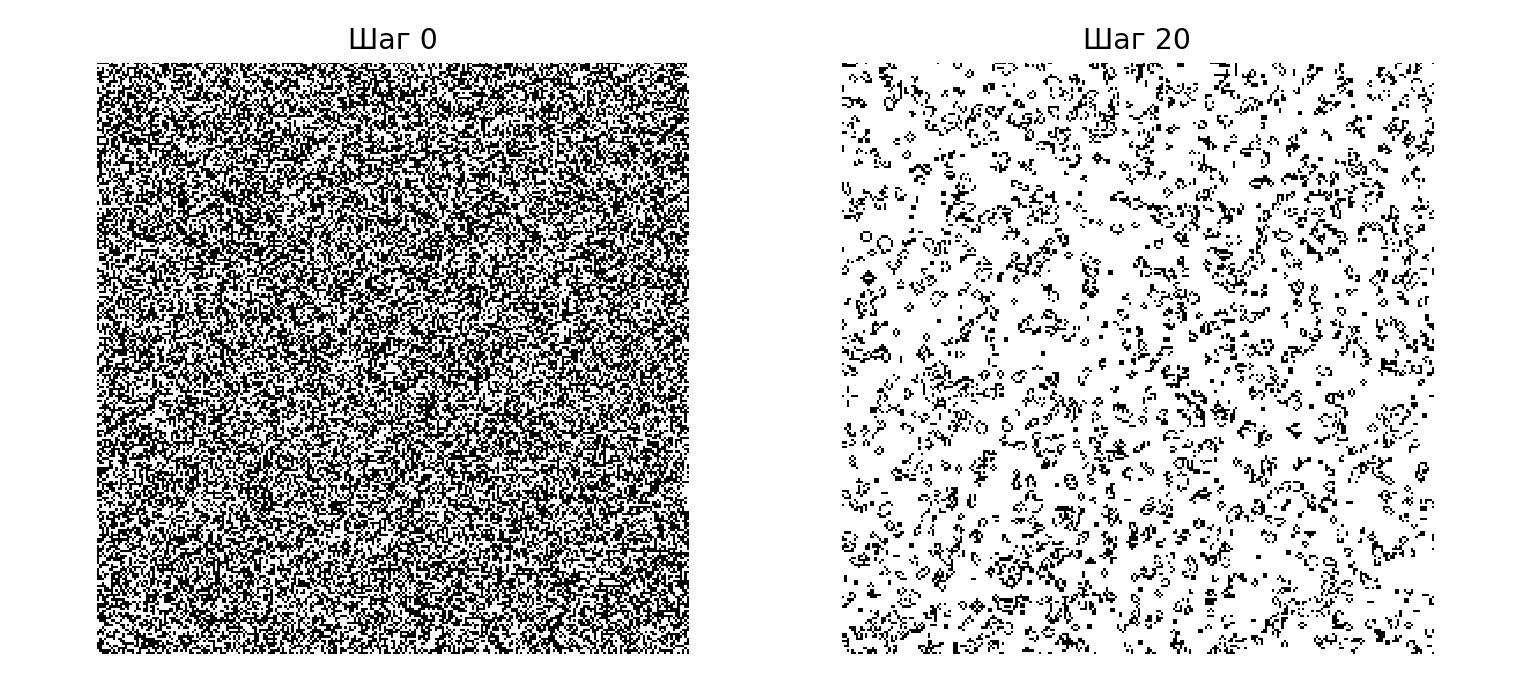
\includegraphics[width=\textwidth]{lab4_evolution.png}
\caption{Начальное поле и результат двадцати поколений}
\end{figure}
\begin{figure}[htbp]\centering
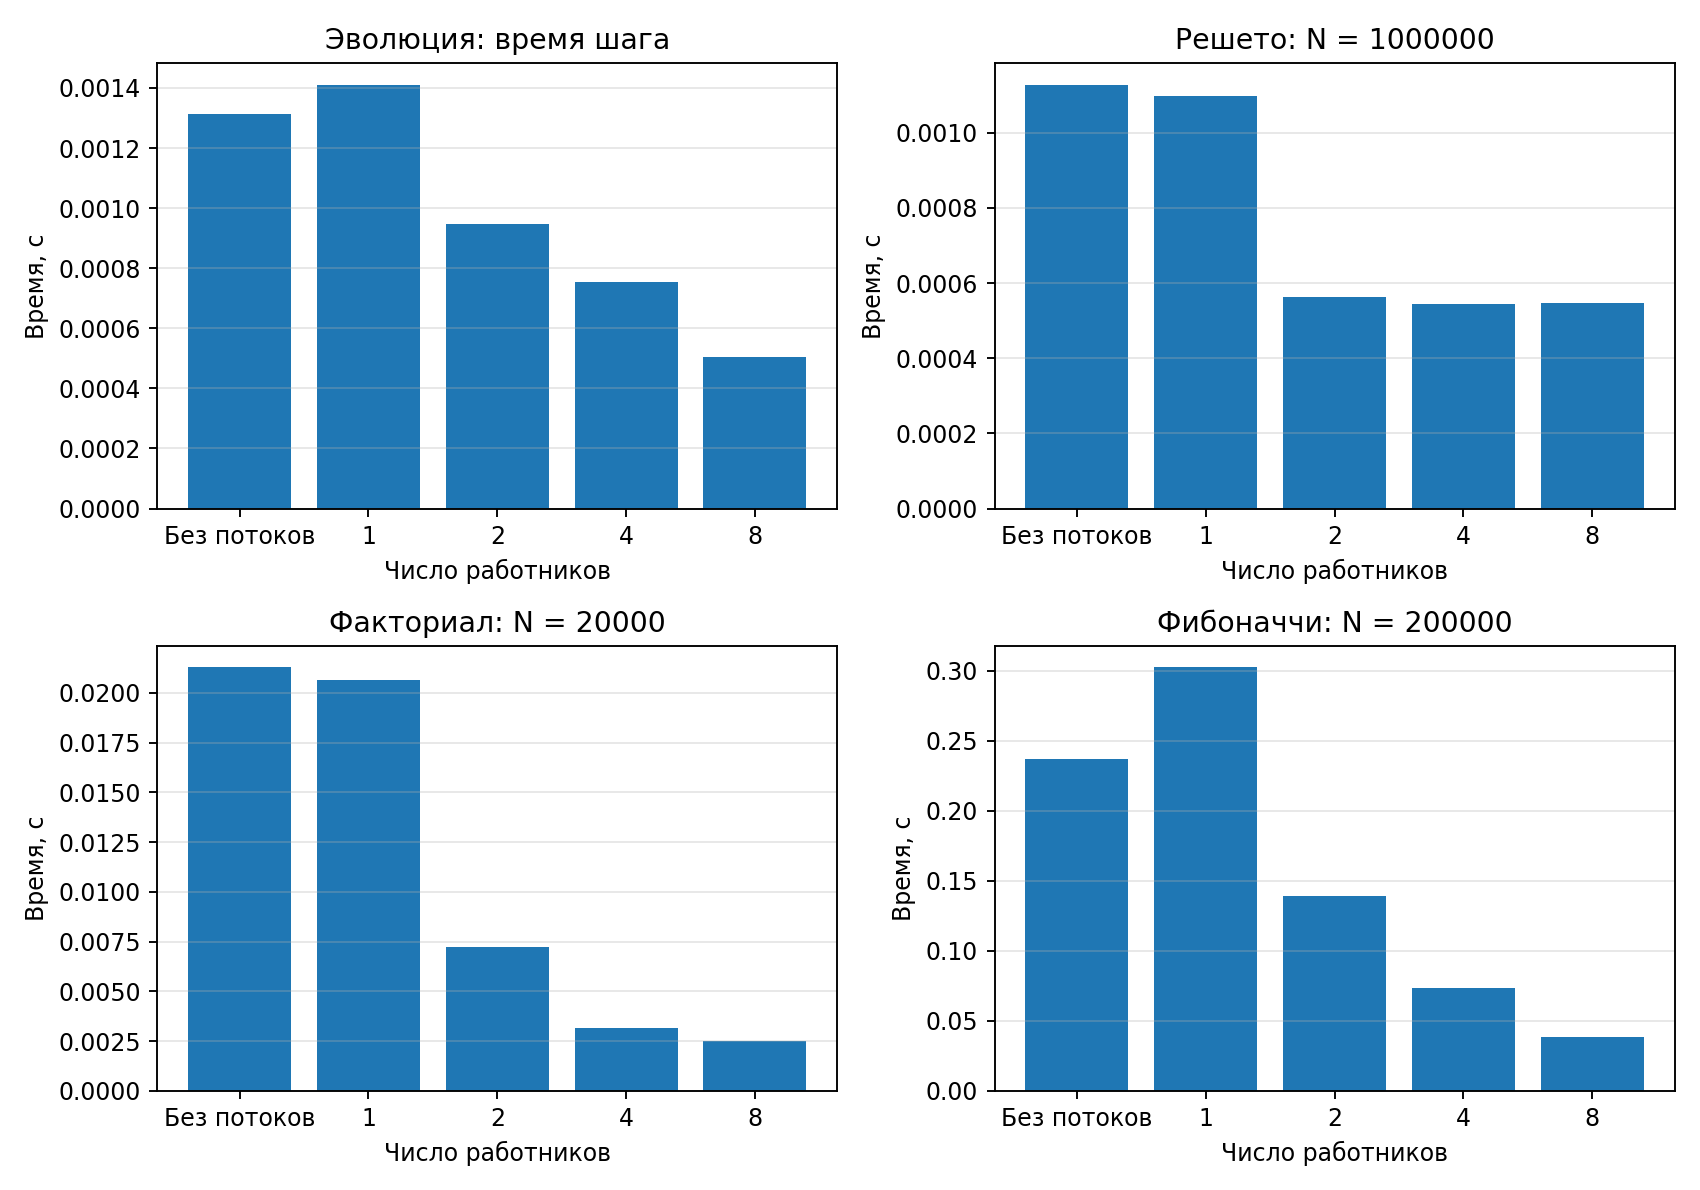
\includegraphics[width=\textwidth]{lab4_times.png}
\caption{Время без работников и при 1, 2, 4, 8 работниках}
\end{figure}

\section{Вывод}
Две программы можно запускать и объяснять независимо.
В задаче 1 обмен граничными строками и барьеры обеспечили одинаковое
поле при разных разбиениях. Восемь работников сократили среднее время
шага примерно с 0.001315 до 0.000504~с.
В задаче 3 сегменты решета исключили пересекающиеся записи.
Вычисления факториала и Фибоначчи также дали правильные ответы.

Факториал и Фибоначчи в этом запуске выиграли от разбиения на части.
Однако оно не только распределяет работу, но и меняет стоимость
арифметики: частичные произведения и последовательности содержат
меньшие целые. Для Фибоначчи дополнительно нужны умножения при
объединении пар. Поэтому весь выигрыш нельзя приписывать только ядрам.

Три замера, особенно коротких операций решета, не доказывают устойчивое
ускорение. На результаты влияют частота процессора, прогрев,
сборка мусора и фоновая нагрузка.

\appendix
\clearpage
\section{Основные фрагменты программы}
В листингах оставлены только алгоритмы и синхронизация.
Объявления пакетов, подготовка исходных данных, измерение времени,
проверки и запись файлов опущены.
Фрагмент обмена строками выполняется внутри рабочего цикла
\texttt{evolution}; это часть функции, а не самостоятельная программа.
Полные исходники находятся в \texttt{task1/main.go} и \texttt{task3/main.go}.

\subsection{Барьер между фазами}
Метод \texttt{wait} защищает счётчики мьютексом и ждёт смены фазы.
Последний участник пробуждает остальных.
\begin{lstlisting}[language=Go,caption={Барьер между фазами}]
func (b *barrier) wait() {
	b.condition.L.Lock()
	defer b.condition.L.Unlock()
	generation := b.generation
	b.arrived++
	if b.arrived == b.total {
		b.arrived = 0
		b.generation++
		b.condition.Broadcast()
	} else {
		for generation == b.generation {
			b.condition.Wait()
		}
	}
}
\end{lstlisting}

\subsection{Обмен границами и шаг эволюции}
Работник запрашивает две соседние строки, отвечает на встречные запросы,
вычисляет новое поколение и проходит две точки синхронизации.
\begin{lstlisting}[language=Go,caption={Обмен границами и шаг эволюции}]
for step := 0; step < steps; step++ {
	requests[(index-1+workers)%workers] <- request{true, topReply}
	requests[(index+1)%workers] <- request{false, bottomReply}
	for k := 0; k < 2; k++ {
		query := <-requests[index]
		row := rows[0]
		if query.last {
			row = rows[len(rows)-1]
		}
		query.reply <- append([]byte(nil), row...)
	}
	next := nextStrip(rows, <-topReply, <-bottomReply)
	phase.wait()
	rows = copyField(next)
	phase.wait()
}
\end{lstlisting}

\subsection{Пул работников}
Работники читают функции из канала до его закрытия.
После отправки всех задач главный поток дожидается их завершения.
\begin{lstlisting}[language=Go,caption={Пул работников}]
func pool(workers int, tasks []func()) {
	jobs := make(chan func())
	var done sync.WaitGroup
	for i := 0; i < workers; i++ {
		done.Add(1)
		go func() {
			defer done.Done()
			for job := range jobs {
				job()
			}
		}()
	}
	for _, task := range tasks {
		jobs <- task
	}
	close(jobs)
	done.Wait()
}
\end{lstlisting}

\subsection{Решето в отдельном сегменте}
Каждая задача изменяет только собственный массив \texttt{marked}.
Общий список базовых простых доступен только для чтения.
\begin{lstlisting}[language=Go,caption={Решето в отдельном сегменте}]
func sieveSegment(start, end int, primes []int) int {
	marked := make([]bool, end-start)
	for _, p := range primes {
		first := max(p*p, ((start+p-1)/p)*p)
		for k := first; k < end; k += p {
			marked[k-start] = true
		}
	}
	for k := end - 1; k >= start; k-- {
		if !marked[k-start] {
			return k
		}
	}
	return 0
}
\end{lstlisting}

\subsection{Факториал с пулом}
Функция \texttt{product(start,end)} перемножает числа полуинтервала
$[start,end)$. Частичные произведения объединяются после завершения пула.
\begin{lstlisting}[language=Go,caption={Факториал с пулом}]
func factorial(n, workers int) *big.Int {
	if workers == 0 {
		return product(1, n+1)
	}
	parts := make([]*big.Int, workers)
	tasks := make([]func(), workers)
	for i := range tasks {
		tasks[i] = func() { parts[i] = product(1+n*i/workers, 1+n*(i+1)/workers) }
	}
	pool(workers, tasks)
	result := big.NewInt(1)
	for _, part := range parts {
		result.Mul(result, part)
	}
	return result
}
\end{lstlisting}

\subsection{Пара соседних чисел Фибоначчи}
Последовательное вычисление пары использует обычный цикл сложений.
\begin{lstlisting}[language=Go,caption={Пара соседних чисел Фибоначчи}]
func fibPair(n int) (*big.Int, *big.Int) {
	a, b := big.NewInt(0), big.NewInt(1)
	for i := 0; i < n; i++ {
		next := new(big.Int).Add(a, b)
		a, b = b, next
	}
	return a, b
}
\end{lstlisting}

\subsection{Фибоначчи с пулом}
Каждая задача вычисляет пару для своей длины блока.
Главный поток объединяет пары по формуле сложения индексов.
\begin{lstlisting}[language=Go,caption={Фибоначчи с пулом}]
func fibonacci(n, workers int) *big.Int {
	if workers == 0 {
		a, _ := fibPair(n)
		return a
	}
	parts := make([][2]*big.Int, workers)
	tasks := make([]func(), workers)
	for i := range tasks {
		tasks[i] = func() {
			parts[i][0], parts[i][1] = fibPair(n*(i+1)/workers - n*i/workers)
		}
	}
	pool(workers, tasks)
	a, b := big.NewInt(0), big.NewInt(1)
	for _, part := range parts {
		c, d := part[0], part[1]
		nextA := new(big.Int).Mul(a, d)
		nextA.Add(nextA, new(big.Int).Mul(new(big.Int).Sub(b, a), c))
		nextB := new(big.Int).Mul(b, d)
		nextB.Add(nextB, new(big.Int).Mul(a, c))
		a, b = nextA, nextB
	}
	return a
}
\end{lstlisting}

\end{document}

